\subsubsection{UC19 - Gioca}
 \begin{figure}[h]
	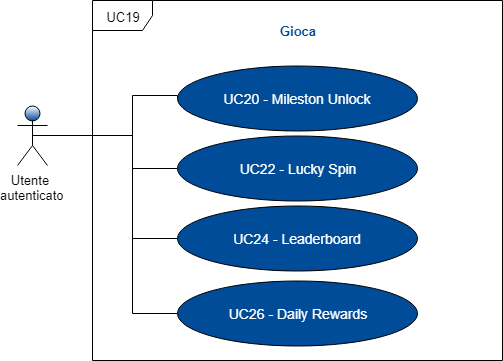
\includegraphics[width=10cm]{res/images/UC19Gioca.png}
	\centering
	\caption{UC19 - Gioca}
\end{figure}
\begin{itemize}
	\item \textbf{Attori Primari}: utente autenticato;
	\item \textbf{Descrizione}: agli utenti autenticati è resa disponibile una maschera che presenta i punti esperienza fino ad ora ottenuti con l'utilizzo dell'applicazione e una lista di tutte le sezioni in cui può ottenere dei premi bonus, quali:
	\begin{itemize}
		\item milestone unlock [UC20];
		\item lucky spin [UC22];
		\item leaderboard [UC24];
		\item daily rewards [UC26];
	\end{itemize} 
	\item \textbf{Scenario principale}: l'utente visualizza i suoi punti esperienza accumulati fino a quel momento e la lista di tutte le sezioni in cui può ottenere dei premi bonus;
	\item \textbf{Precondizione}: l'utente autenticato ha selezionato la voce \textit{Gioca} dal menu dell'applicazione;
	\item \textbf{Post-condizione}: l'utente autenticato ha visualizzato lo storico delle sue prenotazioni concluse. 
\end{itemize} 
